\subsection*{ГЛ12 3/4*}
Докажем что такое преобразование задает гомографию на конике $\varphi_p(A_1) = A_1p \cap C = A_2$ ($C$ -- коника)\\
\textbf{Доказательство}\\
\begin{wrapfigure}{r}{0.4\textwidth}
	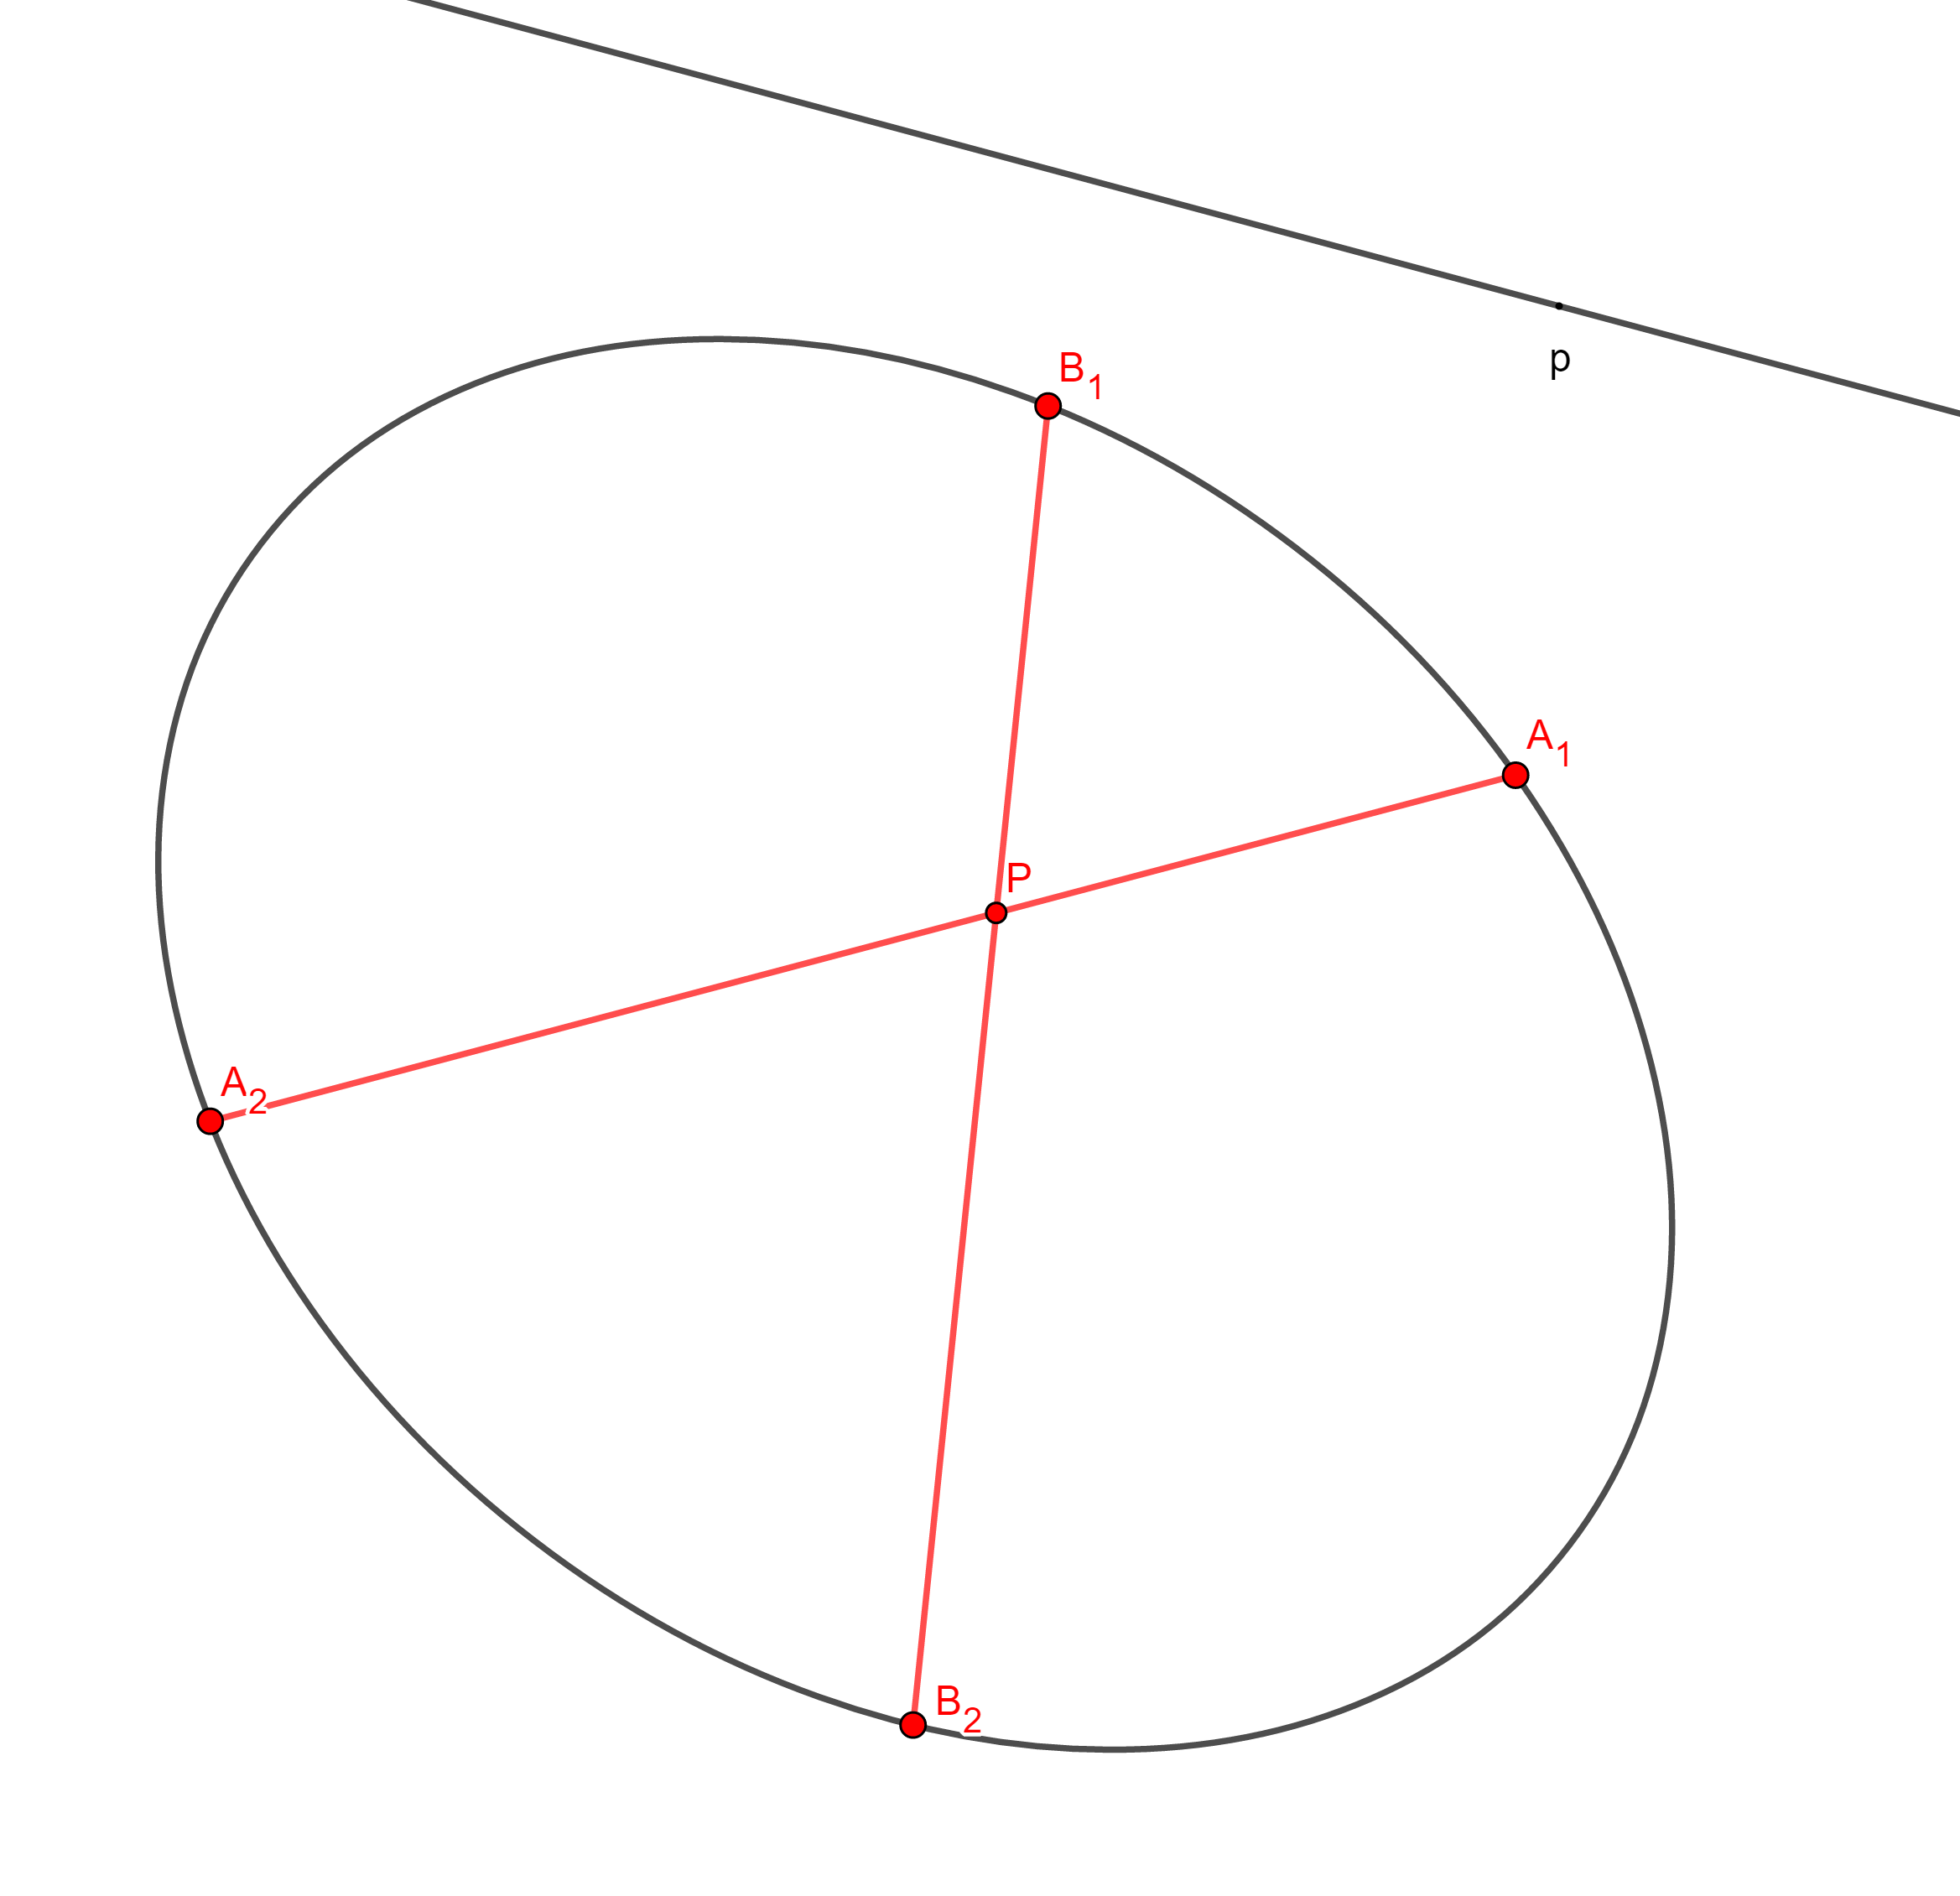
\includegraphics[width=0.8\linewidth]{pic13}
\end{wrapfigure}
Пусть $p_1$ -- поляра точки $p$. $A_1, p, A_2$ лежат на одной прямой, откуда следует что их поляры пересекаются в одной точке, а следовательно $A \in p$, где $A$ -- точка пересечения касательных к конике в точках $A_1, A_2$. Аналогично определим точку $B \in p_1$.\\
Обозначим $A_2B_1 \cap A_1B_2 = X,\ A_1B_1 \cap A_2B_2 = Y$\\
Тогда:
\begin{enumerate}
\item[(1)] по теореме Паскаля для $A_2B_1A_1B_2$ ($B_1, B_2$ двойные),\\ тогда $X,Y,B$ лежат на одной прямой
\item[(2)] по теореме Паскаля для $A_2B_1A_1B_2$ ($A_1, A_2$ двойные),\\ тогда $X,Y,A$ лежат на одной прямой
\end{enumerate}
Тогда так как $A \in p_1,\ B \in p_1$, $A,B,X,Y$ лежат на одной прямой, то $X,Y$ -- лежат на одной прямой $p$, следовательно $\varphi_p$ -- гомография (по задаче $17.13$ из семинара)\\
\begin{figure}[h!]
	\begin{minipage}[h]{0.5\linewidth}
		\center{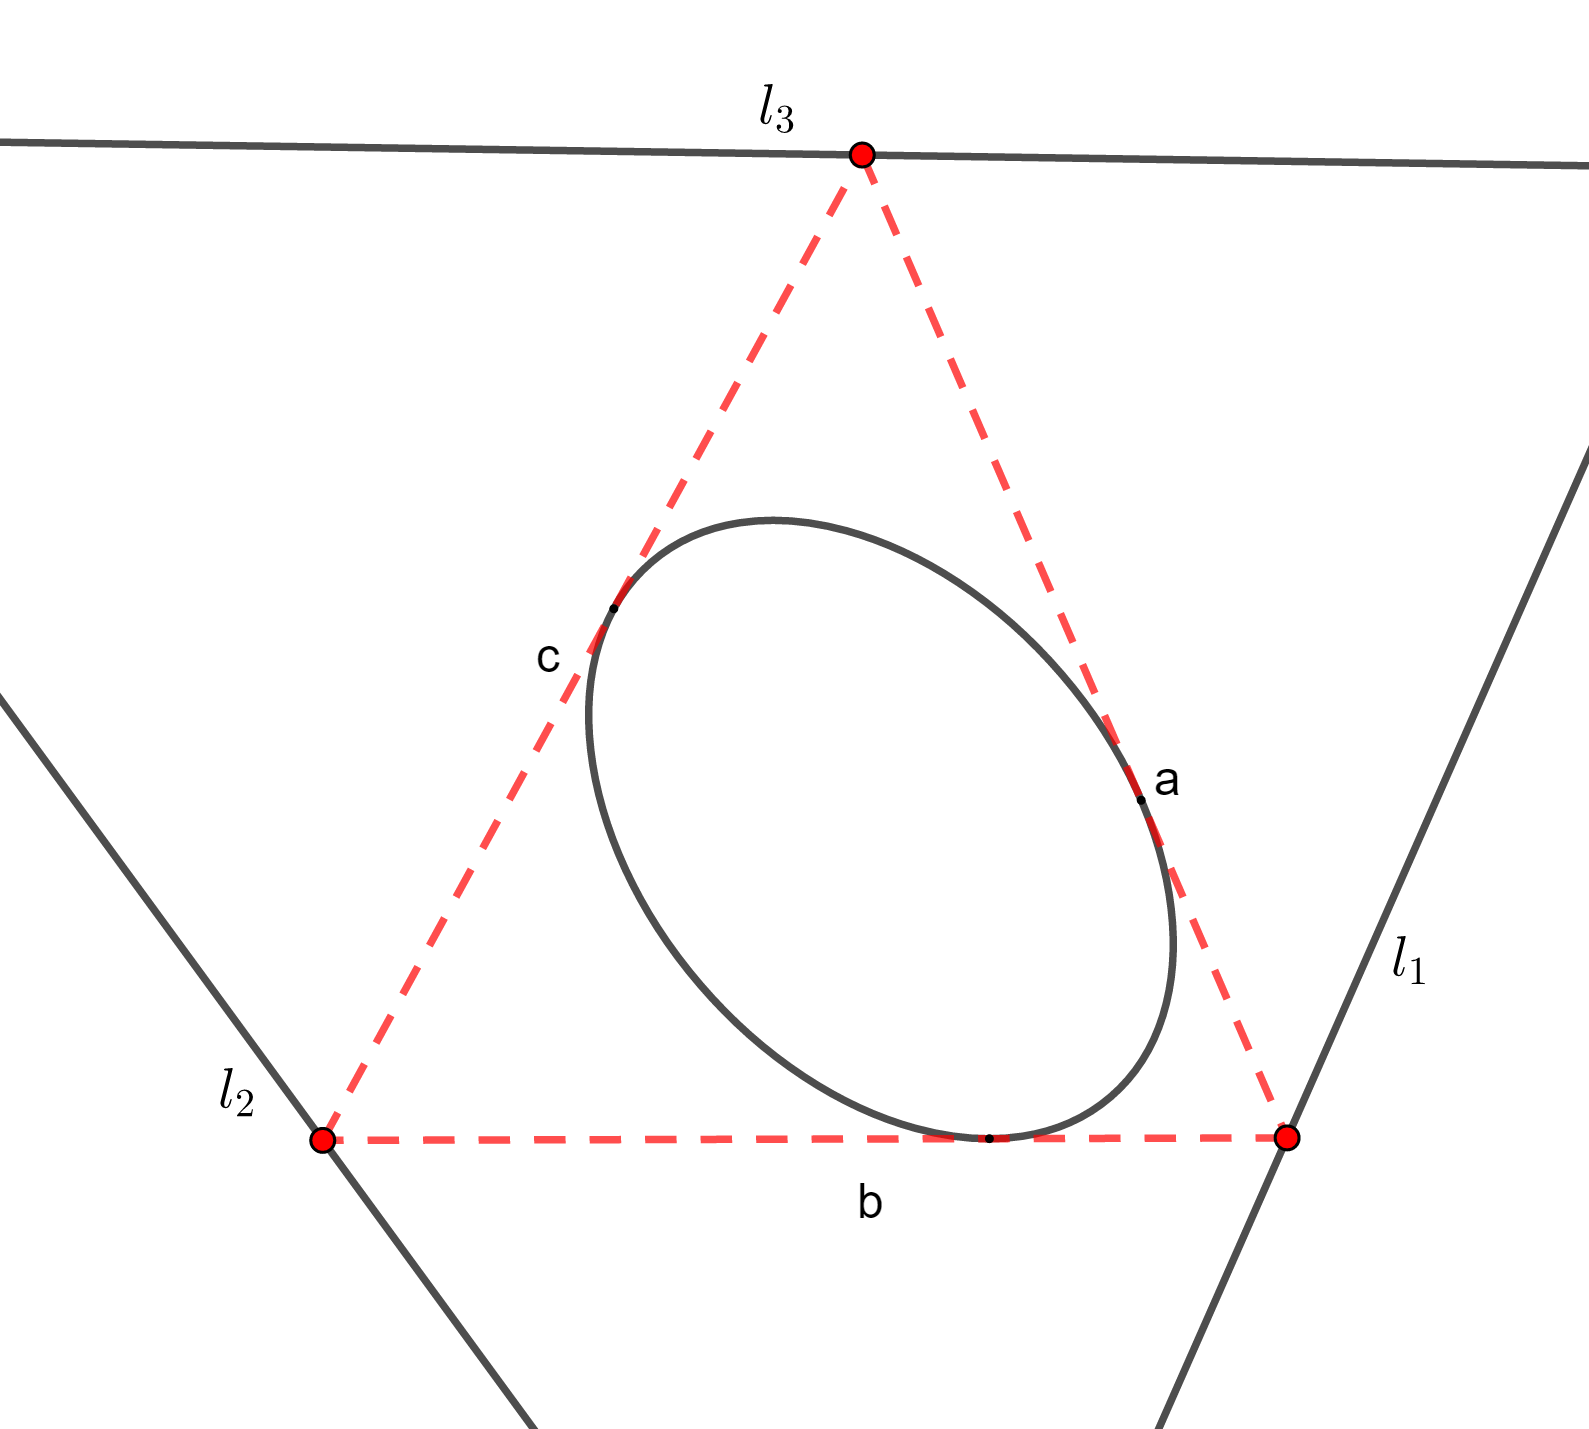
\includegraphics[width=0.5\linewidth]{pic14}}
	\end{minipage}
	\hfill
	\begin{minipage}[h]{0.5\linewidth}
		\center{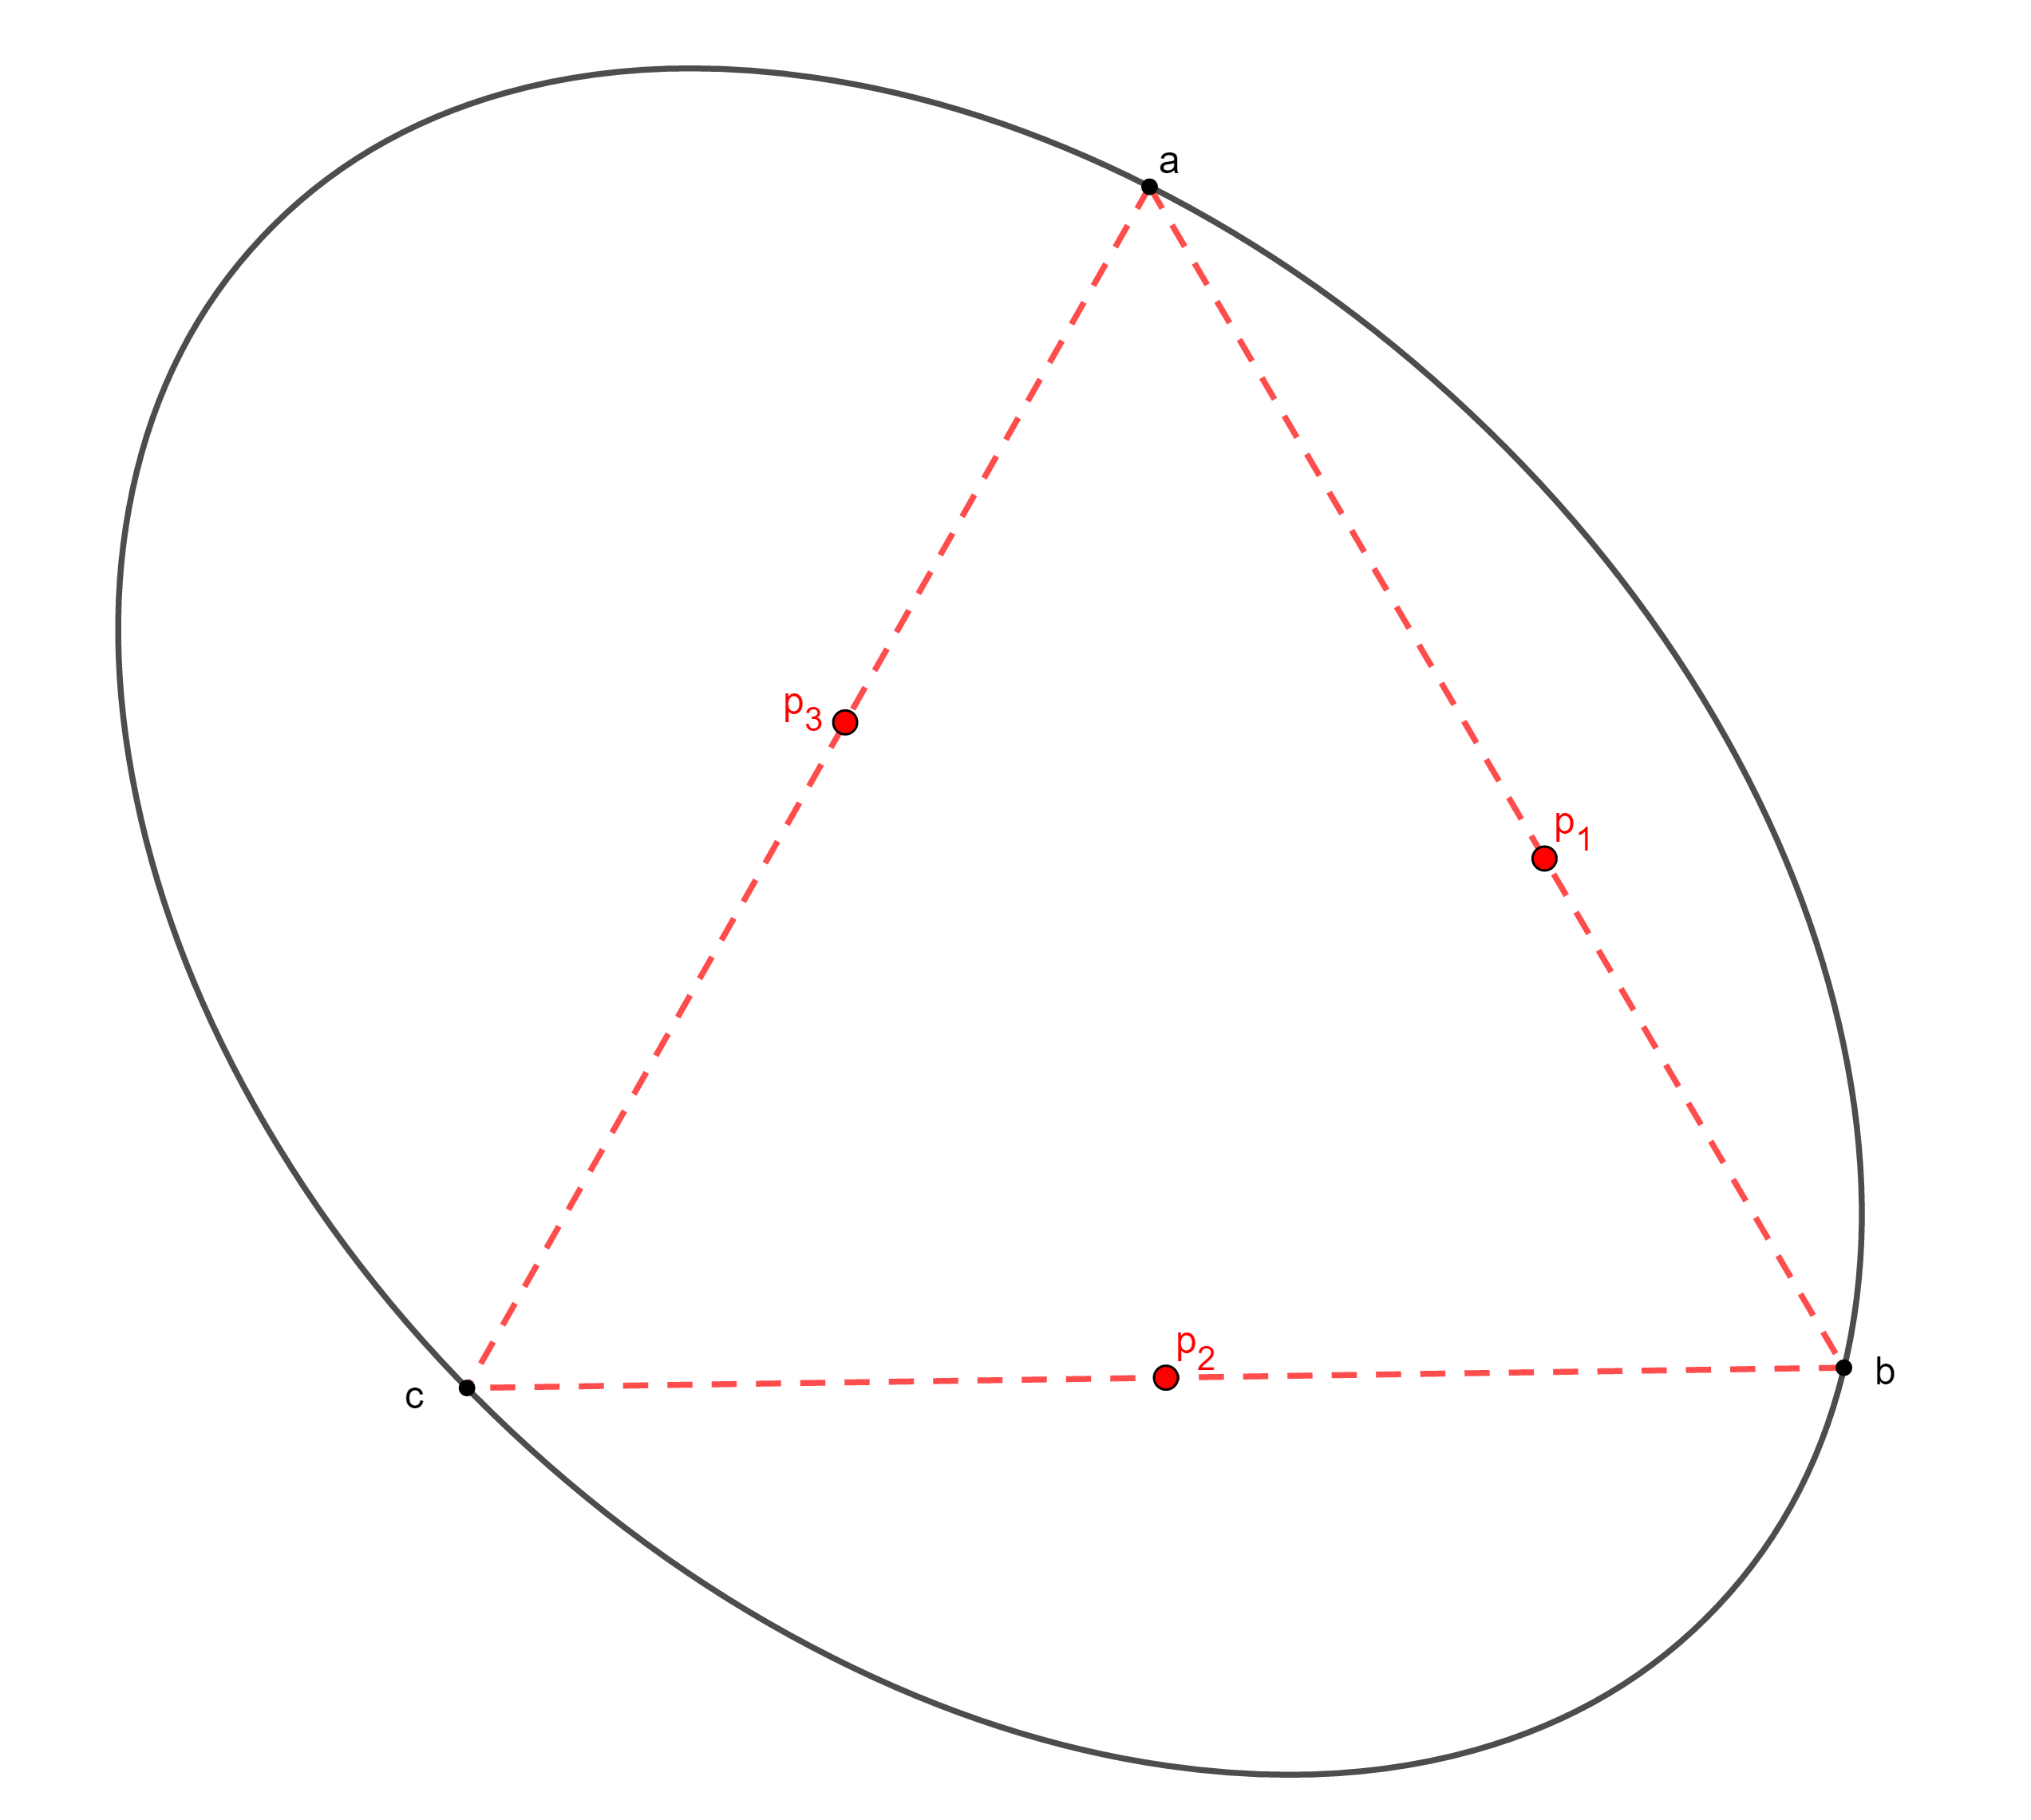
\includegraphics[width=0.5\linewidth]{pic15}}
	\end{minipage}
\end{figure}\\
При замене прямых на их полюсы получим двойственную задачу:\\
$p_1 \to l_1,\ p_2 \to l_2,\ p_3 \to l_3,\ a \to a,\ b \to b,\ c \to c$\\
\\
Докажем двойственное утверждение (ГЛ12 4):\\
\begin{figure}[h!]
	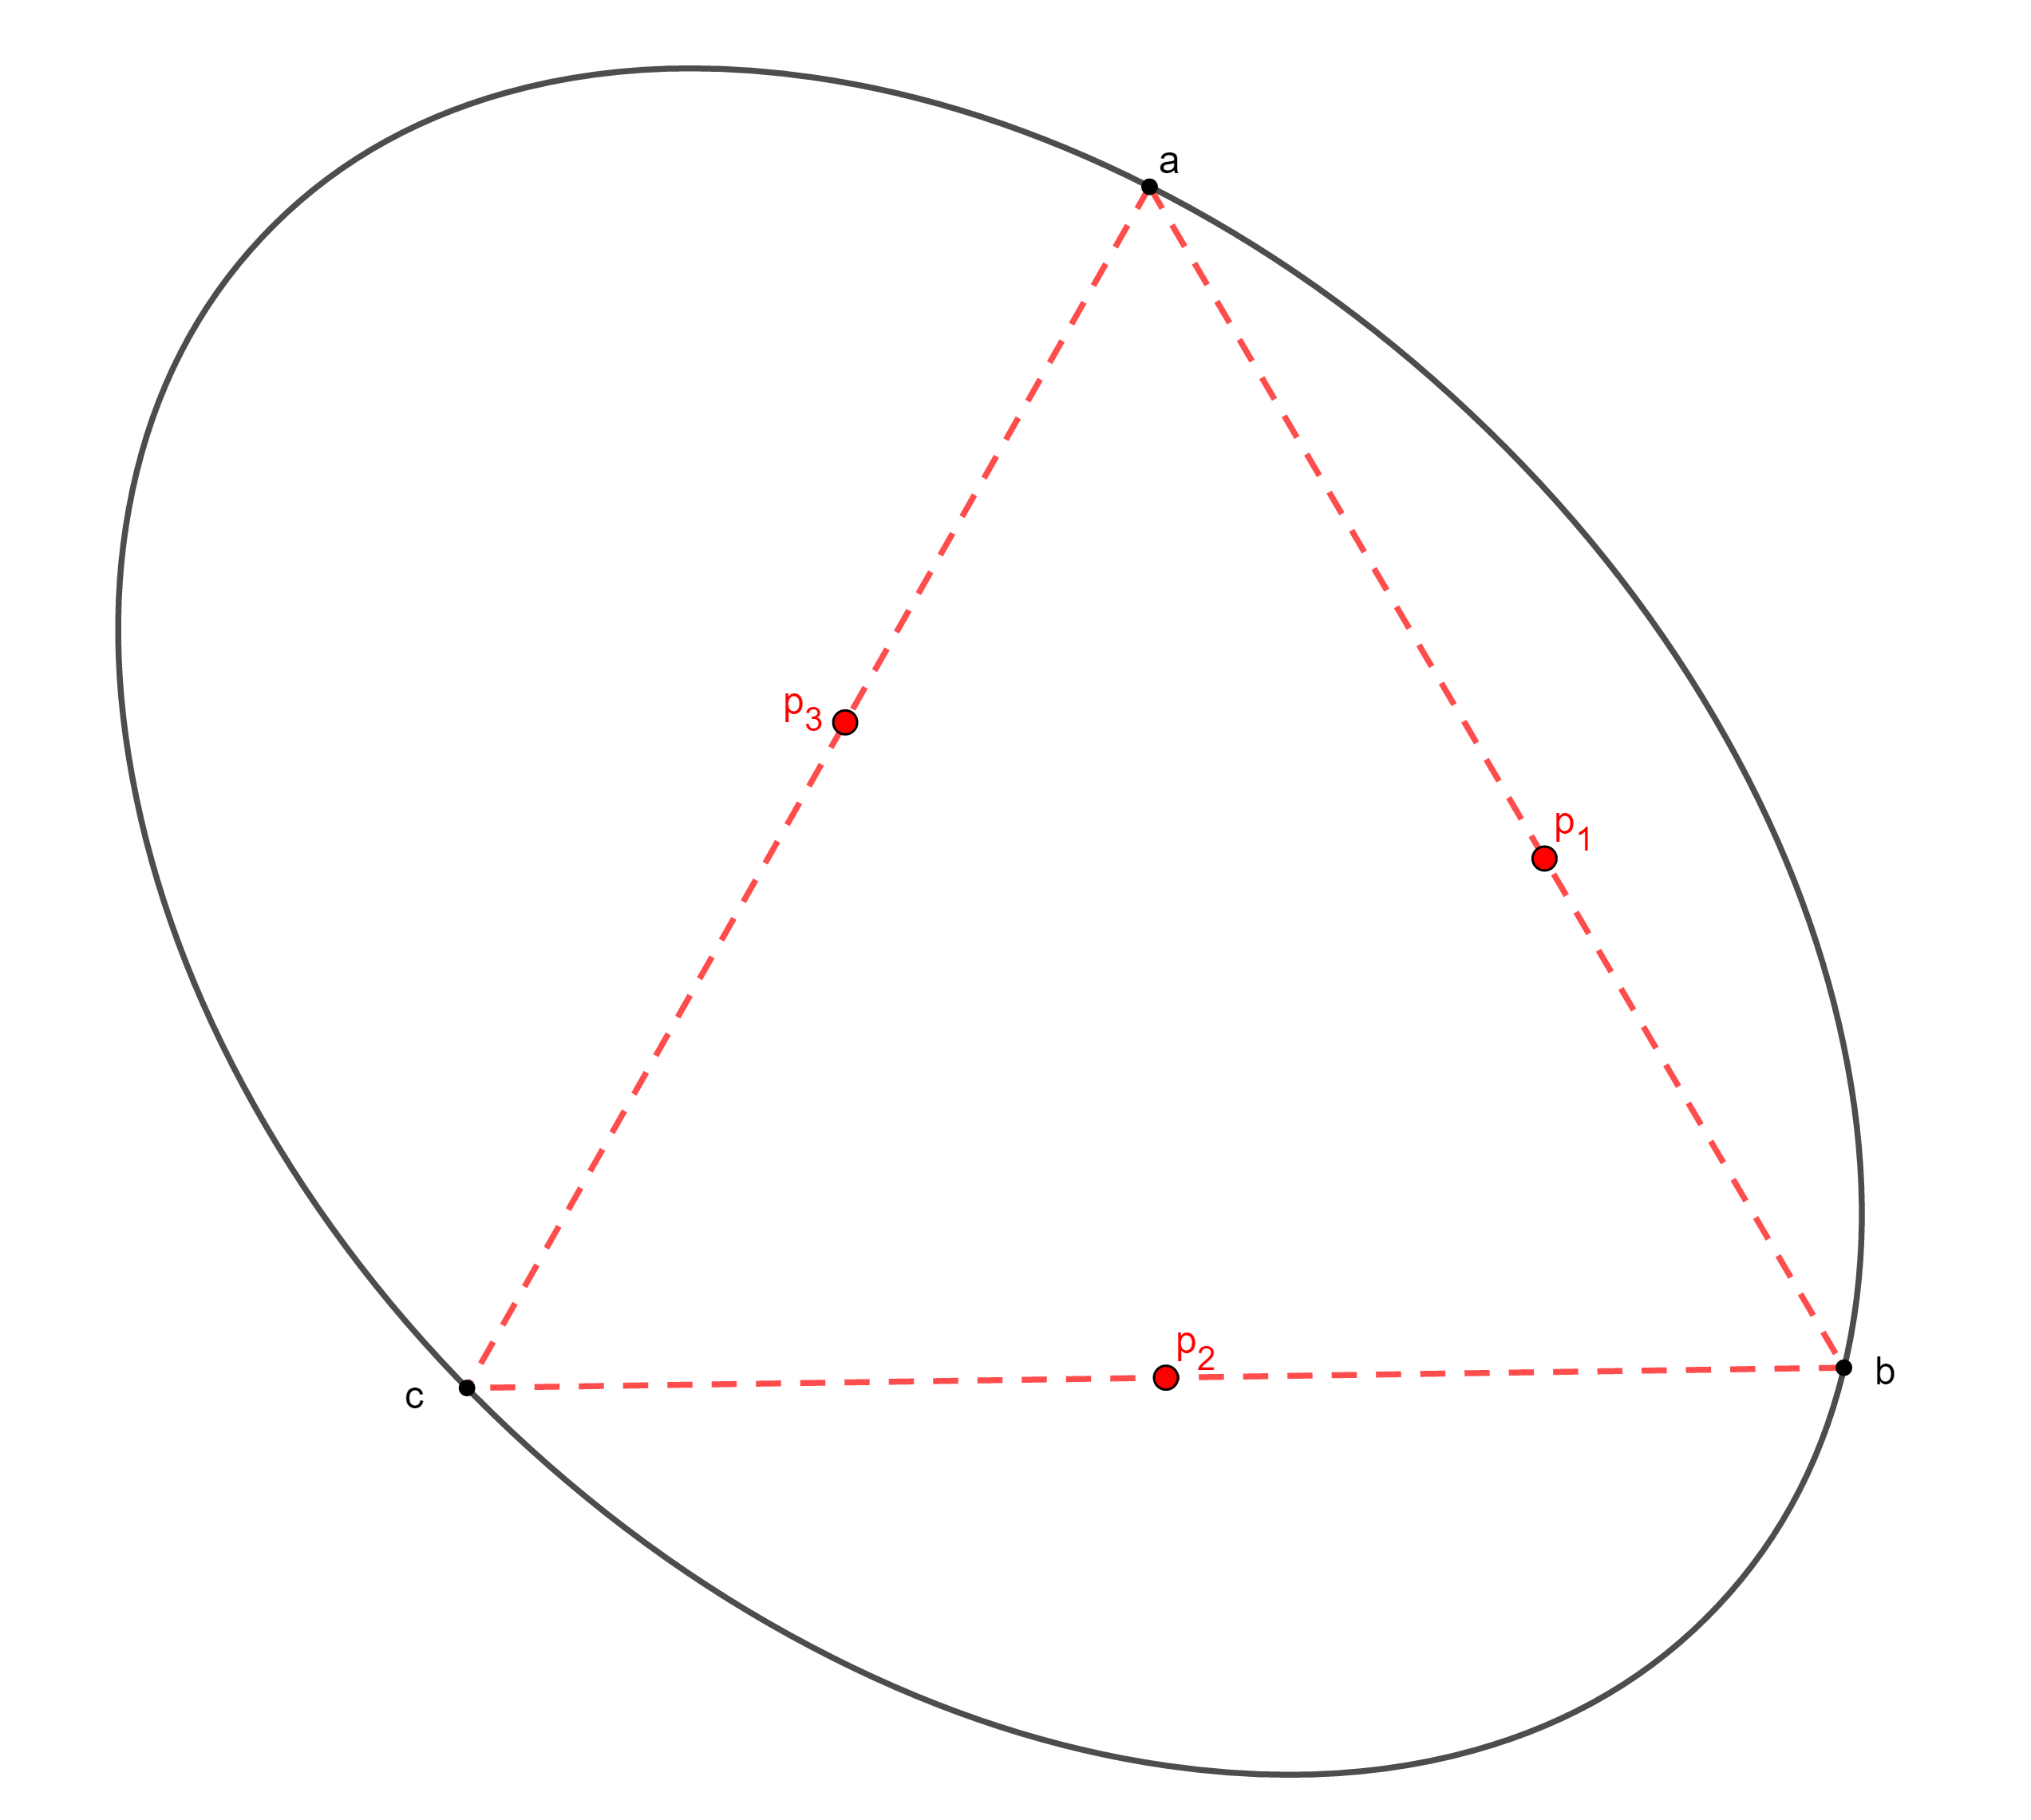
\includegraphics[width=0.3\linewidth]{pic15}
\end{figure}\\
Рассмотрим гомографии $\varphi_{1}, \varphi_{2}, \varphi_{3}$, их композиция тоже гомография $\varphi = \varphi_{1} \circ \varphi_{2} \circ \varphi_{3}$\\
Заметим, что траектория любой неподвижной точки такой гомографии будет давать нам искомый треугольник\\
\vskip 0.2in
\noindent
(по задаче 17.13 из семинаров)\\
Известно, что $\exists \text{ прямая }l,\ \forall A \in C\quad \varphi(A)B \cap \varphi(B)A \in l$\\
А неподвижные точки это $\{l \cap C\} = \{\text{неподвижные точки}\}$ (если $\varphi$ не тождественно), откуда следует что неподвижных точек может быть $0,1,2,\infty$\\
\\
Тогда можно построить образ любой точки и получить прямую $l$, а значит и найти неподвижные точки, если такие существуют.\\
\begin{figure}[!h]
	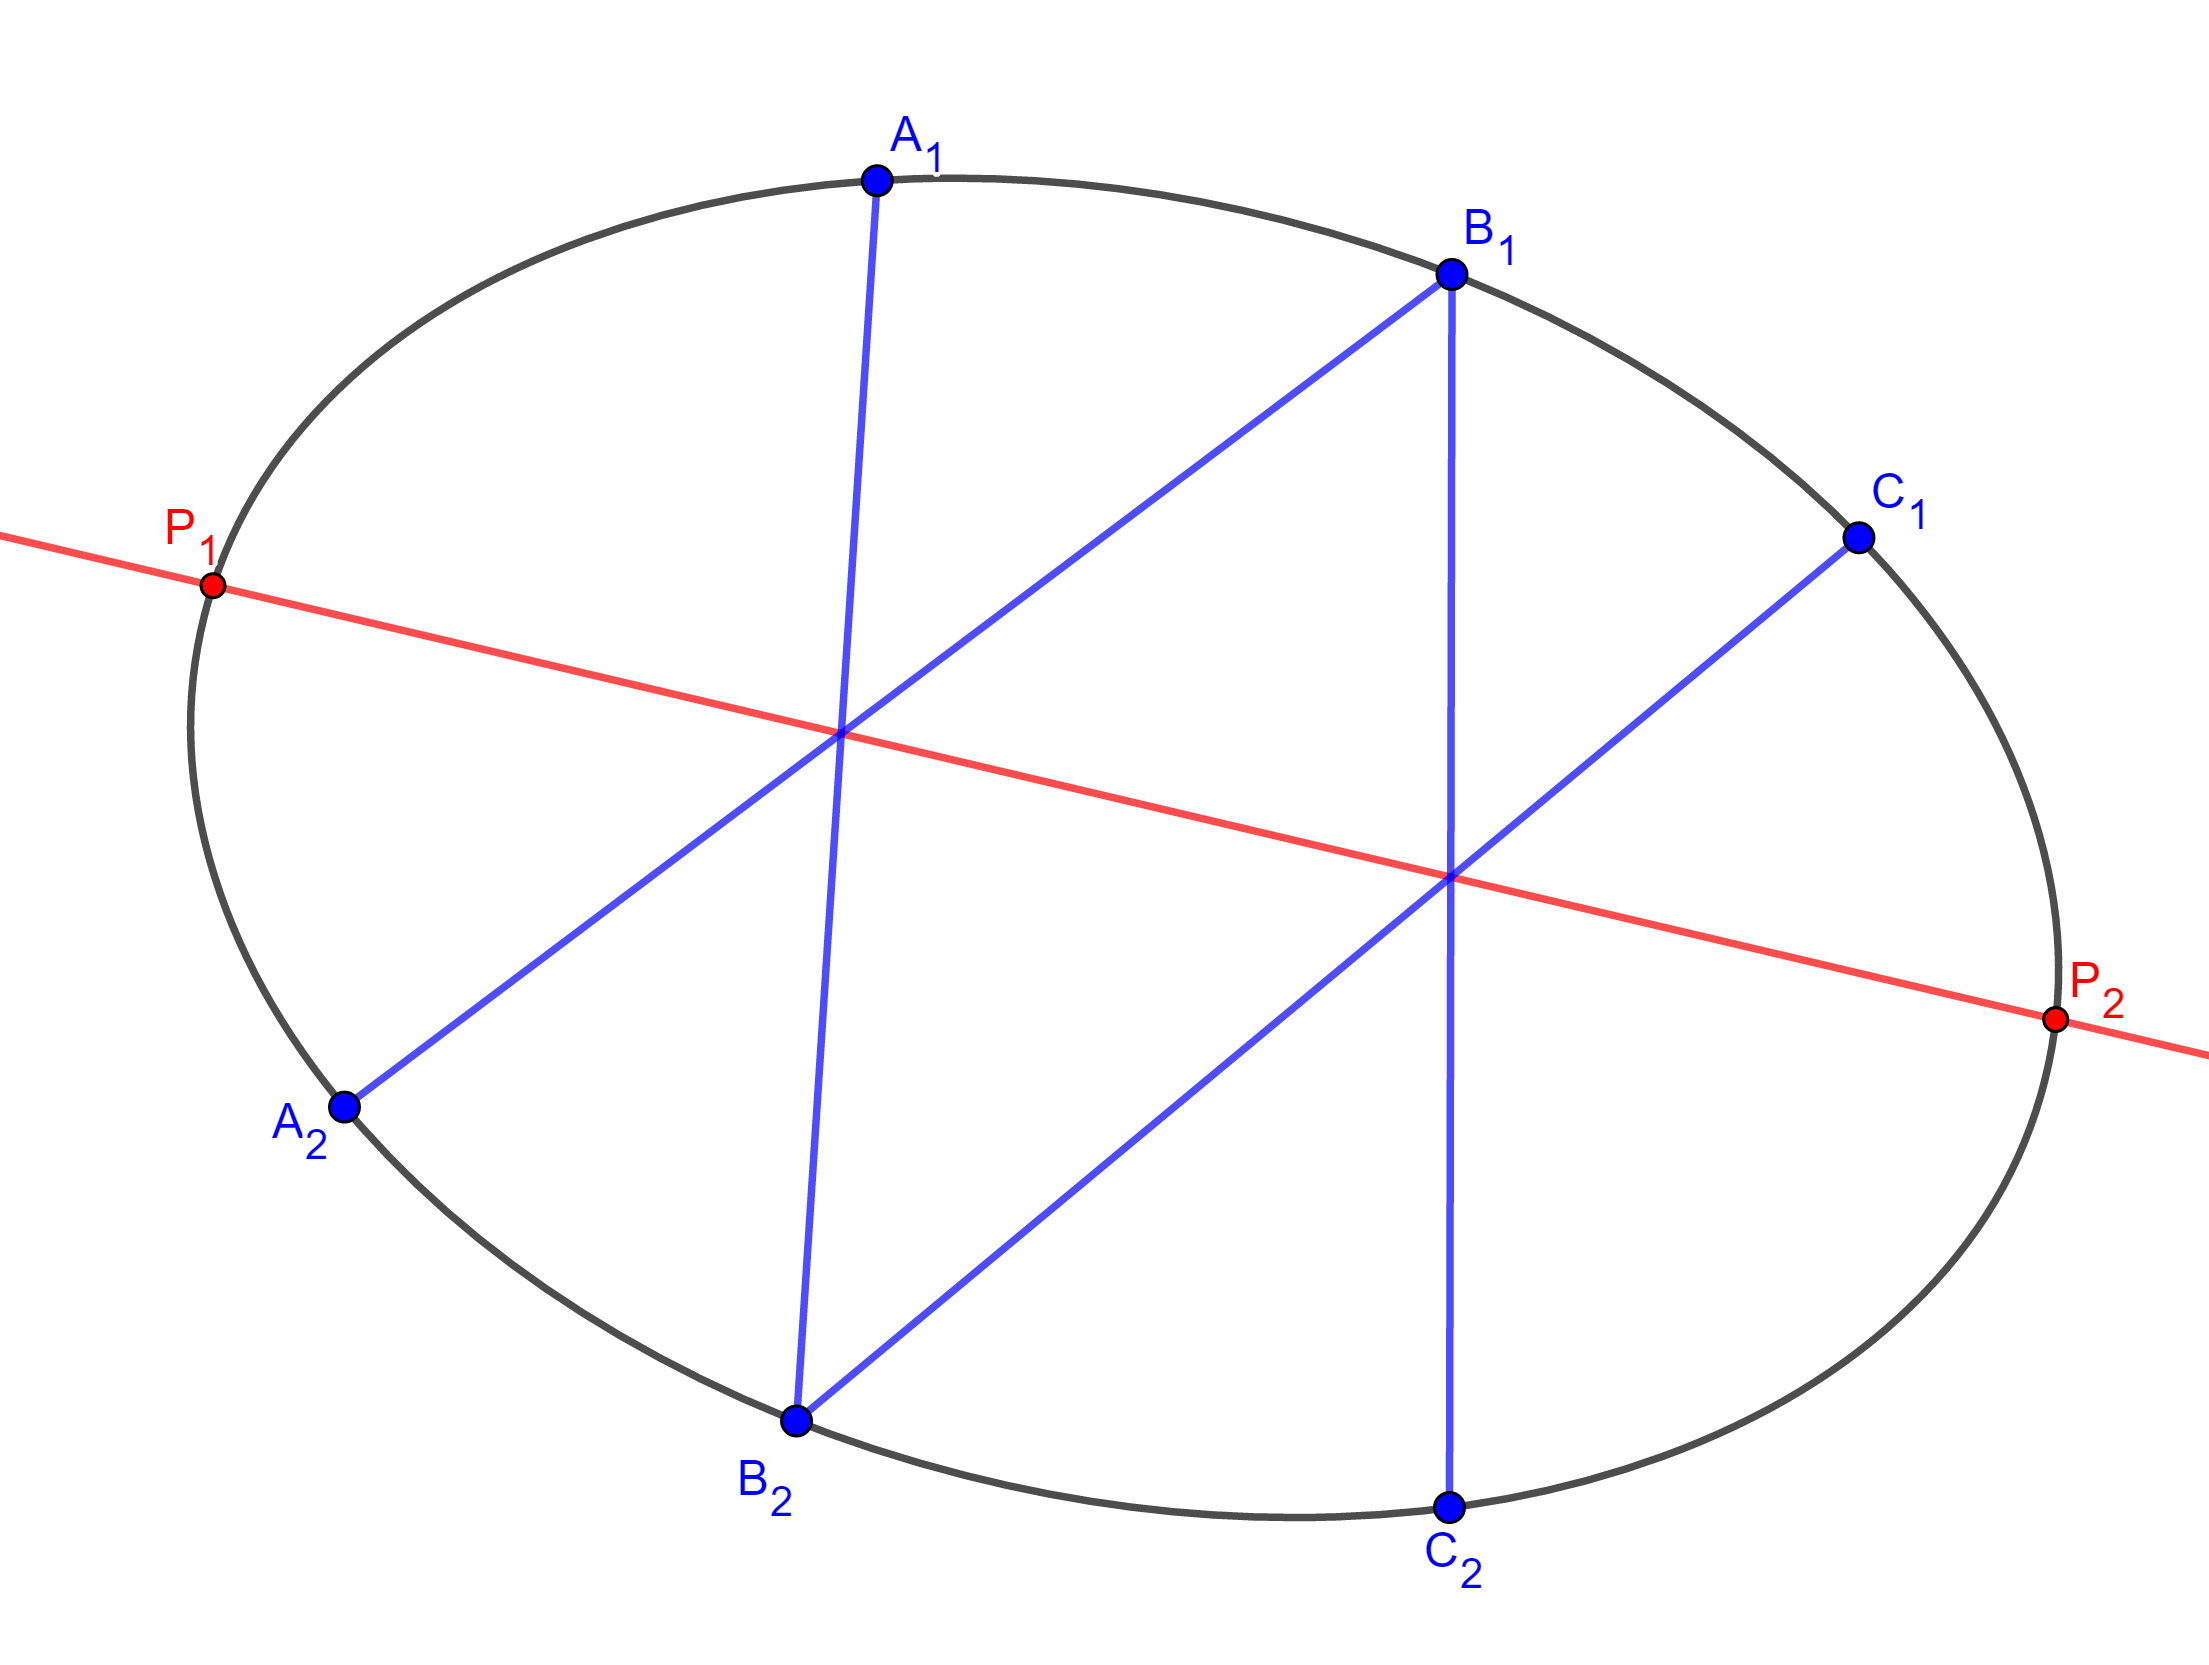
\includegraphics[width=0.5\linewidth]{pic16}
	\text{$p_1, p_2$ -- неподвижные}
\end{figure}\\
Даже по неподвижной точке достраивается треугольник
\begin{figure}[!h]
	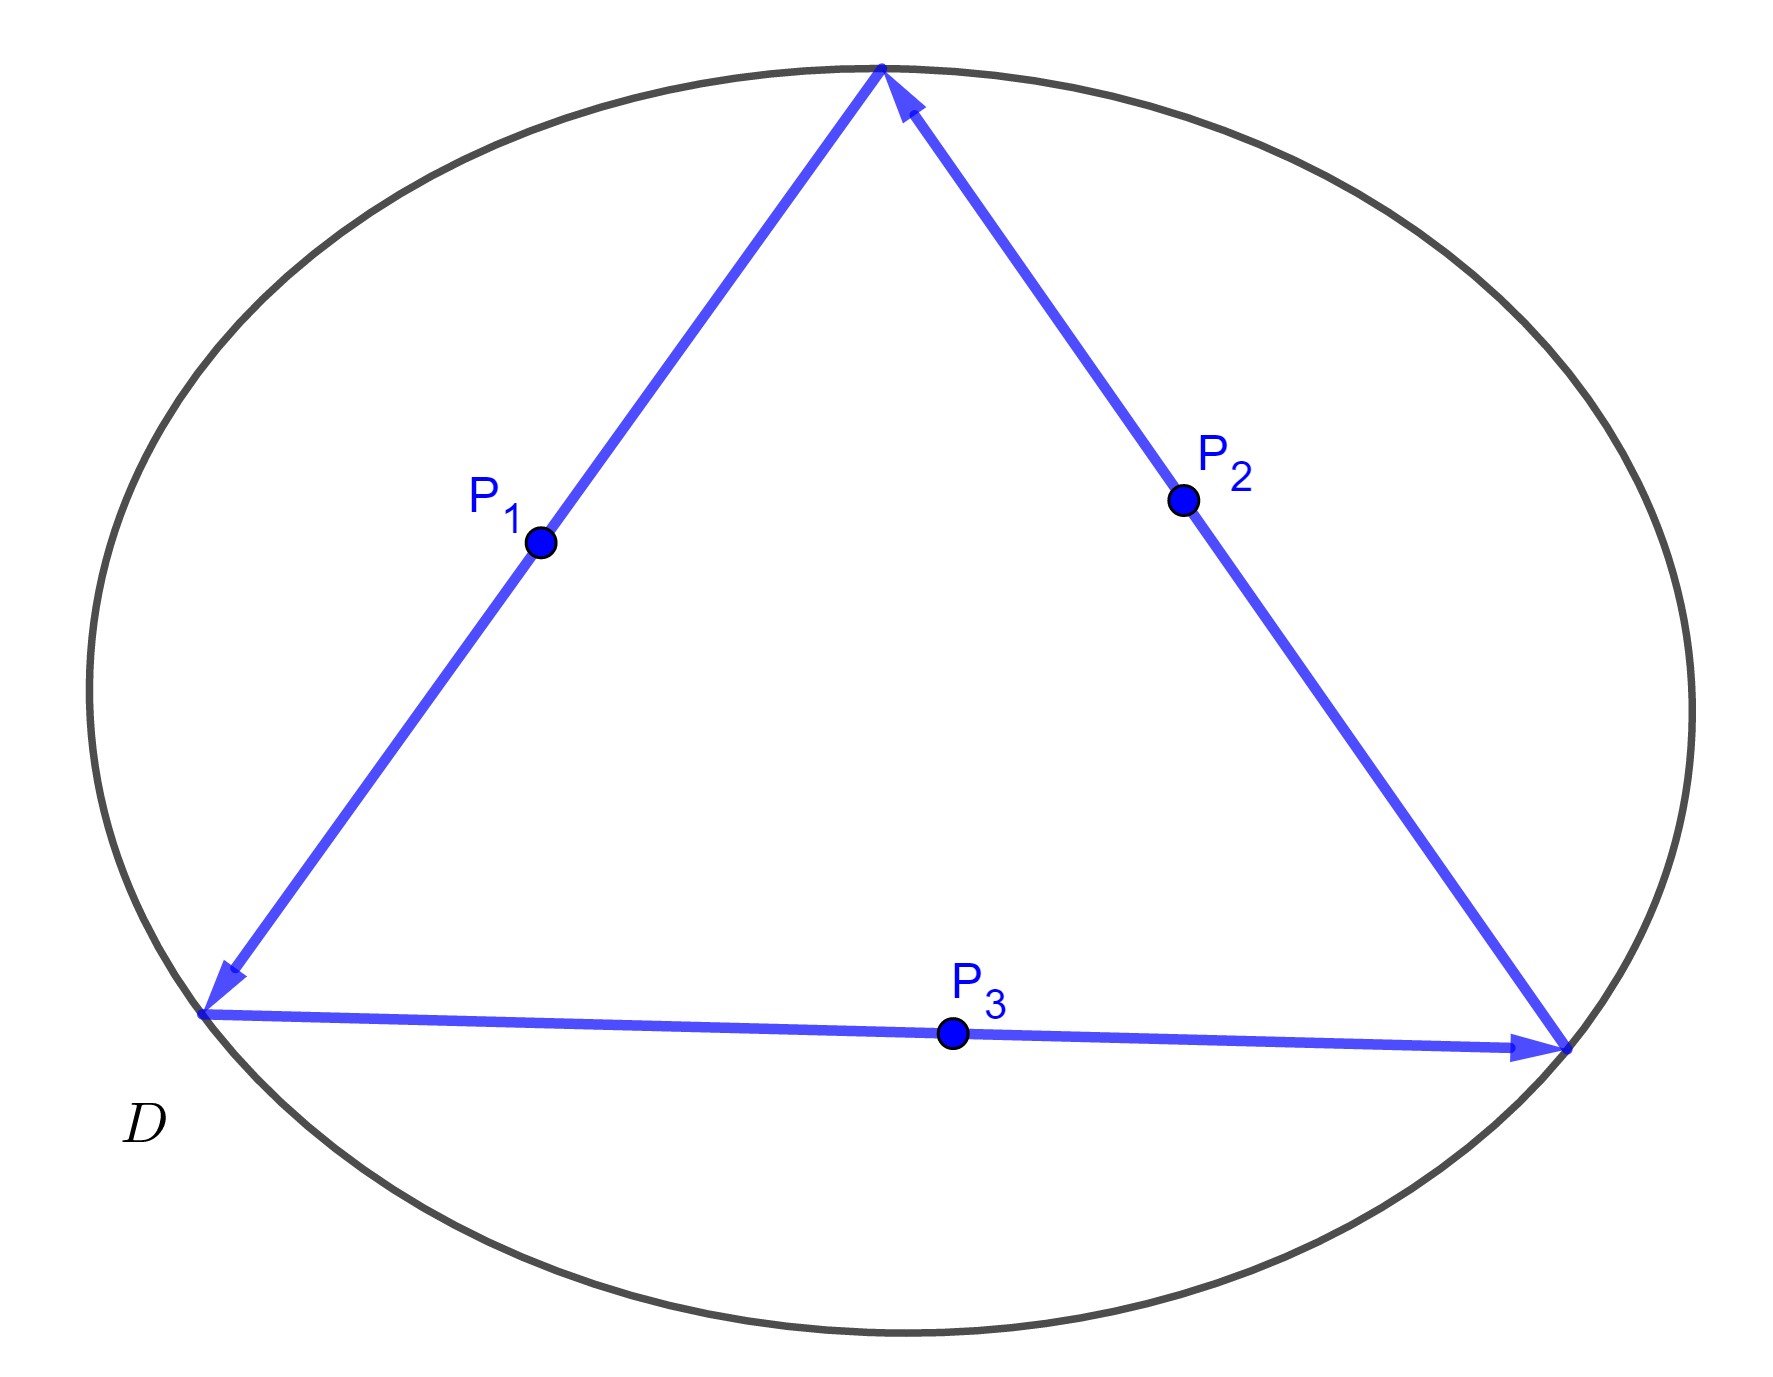
\includegraphics[width=0.5\linewidth]{pic17}
\end{figure}\\
В задаче 3 аналогично показываем что отображение $\varphi_e$:
\begin{gather*}
	X \to \text{касательная в точке $X$ (назовем ее $l_x$)} \to l_x \cap l = A_x\\
	\to \text{вторая касательная $l_{2x}$ к конике из $A_x$} \to l_{2x}\cap C = \varphi(x) \text{ -- гомография}
\end{gather*}
И далее мы проделываем рассуждения аналогичные прошлым